\begin{enumerate}
    \item Purpose \\
          TempoMate's backend serves as the central nervous system, orchestrating seamless communication between users, frontend interfaces, and the intricate web of routines, triggers, and actions within the application. Its overarching purpose is to empower users to effortlessly manage their smart home environment, utilizing real-time video streaming via RTMP to detect user positions and postures, specifically when they are resting in bed. By understanding and interpreting these scenarios, the backend triggers predefined routines, seamlessly executing actions such as turning off room lights. Additionally, the backend administers essential user functionalities, including registration, login, logout, and nickname changes, ensuring a secure and personalized experience for each user. \\\\

    \item Functionality \\
          The backend of TempoMate enhances user experience and enables various functionalities for smart home automation. It efficiently handles user account management tasks, including user registration, authentication (login/logout), and user nickname changes. The core of the app lies in its capability to manage routines, allowing users to define their smart home environment easily through features such as adding, deleting, and sharing routines. Similarly, the backend manages the addition and deletion of actions, enabling users to define specific responses to detected video scenarios. Additionally, the backend facilitates the effective activation of smart home routines by managing the addition and expansion of triggers. Lastly, the backend seamlessly processes real-time video streams captured via RTMP, forwarding them to the frontend and AI components to perform their respective functions. In summary, the multifaceted functionalities of the backend not only ensure a robust user management system but also establish a responsive and adaptive smart home environment based on AI and routines. \\\\

    \item Location of source code \\
          : www.github.com/se-tmp/backend \\\\

    \item Database Implementation\\
          % \begin{enumerate}[label=\alph*]
            \begin{figure*}[!htb]
                \begin{center}
                    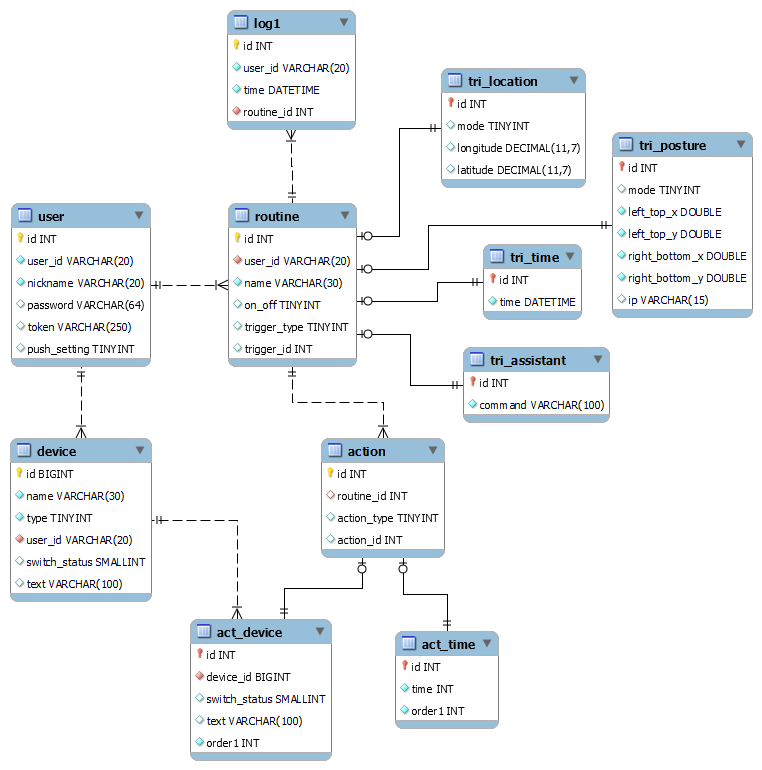
\includegraphics[width=12cm]{imgs/architecture_design_and_implementation/database-erd.png}
                    \caption{Database ERD} 
                    \renewcommand{\thefigure}{\thesubsection.\arabic{figure}}
                \end{center}
            \end{figure*}
          % \addImage{
          %     imgs/architecture_design_and_implementation/database-erd.png
          % }{
          %     Database Diagram
          % }
          This is the database that our architecture is currently using. This database consists of 11 tables. By using the structure of these tables, the data generated by the project can be stored.\\
          \begin{enumerate}
              \item user
                    \begin{itemize}
                        \item Used to store registered user information.
                        \item Primary Key: id (auto-increment, unique identifier in the user table), used for indexing data in the table.
                        \item user\_id: varchar(30), a unique identifier for the user. Used to differentiate between different users in the system.
                        \item nickname: varchar(30), the user's nickname. Displayed on the user interface for personalizing the user experience.
                        \item password: varchar(64), the user's password used for authentication during login. Should be stored encrypted in MD5 format to ensure data security.
                        \item token: varchar(250), the user's token used for authentication and access control, ensuring the security of sensitive operations.
                        \item push\_setting: tinyint, default value 1, push notification settings; 0 indicates disabled, 1 indicates enabled. Controls the status of push notifications in the app.\\
                    \end{itemize}

              \item device
                    \begin{itemize}
                        \item Used to store information about devices connected by users.
                        \item Primary Key: id (auto-increment, unique identifier in the device table), stored in bigint format to accommodate larger device IDs.
                        \item name: varchar(30), the name of the device used for identification and description, allowing users to customize the device name displayed in the app.
                        \item type: tinyint, device type, used for categorizing and distinguishing different types of devices. For example, when it is 1, it represents a sliding light bulb, 2 is a switch light bulb, 3 is a general switch, and so on. Different control components are displayed in the app based on the device type.
                        \item user\_id: varchar(20), linked to the user\_id in the user table, used to identify the owner of the device, ensuring that the device is associated with a specific user.
                        \item switch\_status: smallint, default value 0, represents the on/off status of the device, with values ranging from 0 to 100, indicating the current state of the device.
                        \item text: varchar(100), the device's IP address or command, used for communication and control of the device or for storing other necessary information.\\
                    \end{itemize}

              \item routine
                    \begin{itemize}
                        \item Used to store various routine information saved by users.
                        \item Primary Key: id (auto-increment, unique identifier in the routine table), used for indexing data in the table.
                        \item user\_id: varchar(20), linked to the user\_id in the user table, identifying the owner of the routine, ensuring that the routine is associated with a specific user.
                        \item name: varchar(30), the name of the routine, used to save the user-set routine name.
                        \item on\_off: tinyint, default value 0, the on/off status of the routine, where 0 indicates off and 1 indicates on, controlling the activation status of the routine.
                        \item trigger\_type: tinyint, trigger type, used to indicate which type of trigger will activate this routine. For example, 1 represents location-based triggering, and 2 represents posture recognition triggering.
                        \item trigger\_id: int, linked to the IDs in various trigger tables, used to establish the association between the routine and trigger conditions.\\
                    \end{itemize}

              \item tri\_location
                    \begin{itemize}
                        \item This table is used to store location-based trigger information.
                        \item Primary Key: id (auto-increment, unique identifier in the location trigger table), used for indexing data in the table.
                        \item mode: tinyint, default value 0, mode where 0 represents triggering on entry, and 1 represents triggering on exit. Determines the type of location trigger.
                        \item longitude: decimal(11, 7), longitude representing the coordinates of the location. Used to define the geographic location for location-based triggering.
                        \item latitude: decimal(11, 7), latitude representing the coordinates of the location. Used to define the geographic location for location-based triggering.\\
                    \end{itemize}

              \item tri\_posture
                    \begin{itemize}
                        \item Used to store the screen range to be recognized by the camera.
                        \item Primary Key: id (auto-increment, unique identifier in the posture trigger table), used for indexing data in the table.
                        \item mode: tinyint, default value 0, mode where 0 represents sitting posture triggering, 1 represents standing posture triggering, and 2 represents lying posture triggering. Used to determine the type of posture trigger.
                        \item left\_top\_x: double, the X coordinate of the top-left corner used to define the x-axis of the top-left corner of the posture trigger area. Determines the triggering area for posture recognition.
                        \item left\_top\_y: double, the Y coordinate of the top-left corner used to define the y-axis of the top-left corner of the posture trigger area. Determines the triggering area for posture recognition.
                        \item right\_bottom\_x: double, the X coordinate of the bottom-right corner used to define the x-axis of the bottom-right corner of the posture trigger area. Determines the triggering area for posture recognition.
                        \item right\_bottom\_y: double, the Y coordinate of the bottom-right corner used to define the x-axis of the bottom-right corner of the posture trigger area. Determines the triggering area for posture recognition.
                        \item ip: varchar(15), can be used for the camera's IP address if needed.\\
                    \end{itemize}

              \item tri\_assistant
                    \begin{itemize}
                        \item Used to store characters or sentences that need to be recognized.
                        \item Primary Key: id (auto-increment, unique identifier in the assistant trigger table), used for indexing data in the table.
                        \item command: varchar(100), can be used to store an IP address or command for voice recognition.\\
                    \end{itemize}

              \item tri\_time
                    \begin{itemize}
                        \item Used to store the time required for time triggers.
                        \item Primary Key: id (auto-increment, unique identifier in the time trigger table).
                        \item time: datetime, stores the trigger time, used to specify when operations related to this time should be triggered.\\
                    \end{itemize}

              \item action
                    \begin{itemize}
                        \item Serves as the main table for actions, allowing data related to actions to be retrieved based on their types and IDs.
                        \item Primary Key: id (auto-increment, unique identifier in the action table), used for indexing data in the table.
                        \item routine\_id: int, linked to the ID in the routine table, indicating the routine associated with this action. Establishes the association between actions and routines.
                        \item action\_type: tinyint, action type, where 1 represents device actions and 2 represents time-delayed time actions. Used to determine the type of action.
                        \item action\_id: int, linked to the ID in the corresponding action type table. Using the action type data and action ID, specific information about the action can be retrieved.\\
                    \end{itemize}

              \item act\_device
                    \begin{itemize}
                        \item Used to store the state to which devices should be changed after action triggers.
                        \item Primary Key: id (auto-increment, unique identifier in the device action table), used for indexing data in the table.
                        \item device\_id: bigint, linked to the ID in the device table, indicating the device to be controlled. Establishes the association between actions and devices.
                        \item switch\_status: smallint, default value 0, represents the switch status to be modified by the action, with values ranging from 0 to 100.
                        \item text: varchar(100), used to store the device's IP address or command, specifying the specific operation of the device action.
                        \item order1: int, indicates the order in which the action should be executed. Used to determine the execution order when multiple actions are present.\\
                    \end{itemize}

              \item act\_time
                    \begin{itemize}
                        \item Stores the specific time for delayed triggers.
                        \item Primary Key: id (auto-increment, unique identifier in the time action table), used for indexing data in the table.
                        \item time: int, time in seconds, indicating the time delay for executing the action. Used to specify the triggering time for time actions.
                        \item order1: int, indicates the order in which the action should be executed. Used to determine the execution order when multiple actions are present.\\
                    \end{itemize}

              \item log1
                    \begin{itemize}
                        \item Stores log trigger records.
                        \item Primary Key: id (auto-increment, unique identifier in the log table), used for indexing data in the table.
                        \item user\_id: varchar(20), linked to the user\_id in the user table, indicating the user to whom the log belongs. Ensures that the log is associated with a specific user.
                        \item time: datetime, records the time the log was generated. Used to track the time of events.
                        \item routine\_id: int, linked to the ID in the routine table, indicating the routine associated with the log. Used to indicate which routine triggered this log record.\\
                    \end{itemize}

          \end{enumerate}
    \item Class Component \\
    \item[-] pom.xml: This file is associated with the Maven build management tool commonly used in Java projects. It contains project configuration information and is written in XML format. It is used to define project settings, dependencies, plugins, and other build-related information.\\
    \item[-] src/main/resources/application.properties : This configuration file defines settings for a Spring Boot application, specifying the context path as "/api" and providing connection details for a MySQL database.\\
    \item[-] src/main/java/com.tempomate/controller: This is the folder that contains controllers which handle user input and return the results to the user. \\
    \item[-] ActionController: This class handles API operations related to actions using POST, GET, and DELETE mappings. The "/actDevice\_add" and "/actTime\_add" endpoints use POST requests to respectively add device actions and time delay actions. The "/get\_all\_action/\{userId\}" endpoint retrieves all actions stored in the database using a GET request, where \{userId\} is the user identifier. The "/delete/\{id\}" endpoint deletes the action corresponding to the provided ID from the database using a DELETE request.\\
    \item[-] DeviceController: This class handles various mappings related to devices, including POST, DELETE, GET, and PUT. The "/add" endpoint uses POST to add a device to the database. The "/delete/\{id\}" endpoint, using DELETE, removes the device with the specified ID from the database. The "/get\_all\_device/\{userId\}" endpoint, with GET, returns all devices associated with the given user ID. The "/rename\_device" endpoint, using PUT and receiving a new device name in the request body, updates the device name. Lastly, the "/change\_status" endpoint, through PUT, receives a request to change the device's switch within the range of 0 to 100. \\
    \item[-] LogController: This class handles logging, and the "/user/\{userId\}" endpoint, through a GET mapping, returns a list of all logs for the user corresponding to the user ID in the endpoint. \\
    \item[-] RoutineController: This class handles various mappings related to routines, encompassing POST, DELETE, GET, and PUT methods. The "/add" endpoint is used to create a new routine using a POST request. The "/delete/\{id\}" endpoint, through a DELETE mapping, processes the deletion of the routine associated with the provided ID. The "/get\_all\_routine/\{userId\}" endpoint, utilizing the GET method, returns a list of all routines associated with the specified `\{userId\}` value. The "/rename\_routine" endpoint, receiving a request for a new routine name, updates the routine's name using a PUT request. Finally, the "/change\_status" endpoint, taking the routine's ID and on/off status in the request body, updates the routine's on/off status using a PUT request. \\
    \item[-] TriggerController: This class uses POST mappings to add triggers and GET mappings to retrieve them. The endpoints "/loc\_add," "/pos\_add," "/assi\_add," and "/time\_add" are used to respectively add location triggers, posture triggers, assistant triggers, and time triggers through POST requests. The "/get" endpoint receives triggerType and triggerId in the request and returns the corresponding trigger using a POST mapping. Additionally, conditional statements are used to fetch different triggers based on the trigger type of the routine. For each trigger type, it retrieves the appropriate trigger (TriLocation, TriPosture, TriAssistant, TriTime) from the database. \\
    \item[-] UserController: This class handles user-related information using POST and PUT mappings. The "/signup" endpoint deals with user registration using a POST request. The "/login" endpoint is a POST API that receives the user's ID and password in the request for performing login. The "/rename-nickname" endpoint updates the user's nickname by receiving a new nickname through a PUT request. The "/push\_setting" endpoint manages the user's push notification status using a PUT request.\\
    \item[-] src/main/java/com.tempomate/exception/ \par GlobalExceptionHandler: This code defines a global exception handler in a Spring Boot application.\\
    \item[-] src/main/java/com.tempomate/mapper : This is the folder that is employed to define and execute SQL queries for interacting with a database. \\
    \item[-] ActionMapper: This interface interacts with the database to provide functionality related to actions. The `addAction`, `addActDevice`, and `addActTime` methods are responsible for adding action, device action, and time delay action, respectively, to the database. The `getActDevice` and `getActTime` methods retrieve device actions and time delay actions associated with a user and routine. Lastly, the `deleteAction` method removes all action data from the database. \\
    \item[-] DeviceMapper: This interface handles database operations for the `Device` entity. It includes methods to add a new device, retrieve all devices associated with a specific user, delete a device based on its ID, rename a device, and update the switch status of a device. \\
    \item[-] LogMapper : This interface handles database retrieval operations related to the `Log` entity. The `get\_all\_log` method retrieves all logs associated with a specific user ID from the database.\\
    \item[-] RoutineMapper: This interface manages database operations related to the `Routine` entity. It includes methods for adding a new routine, deleting a routine based on a specific ID, renaming a routine, and updating the active/inactive status of a routine. \\
    \item[-] TriggerMapper: This interface is responsible for handling database operations related to triggers in the context of routines. This includes methods for adding triggers of different types (location, posture, assistant, and time) and retrieving specific trigger information based on the trigger ID associated with a routine. \\
    \item[-] UserMapper: This interface handles database operations related to user management. It includes methods for retrieving a list of users (primarily used for testing purposes), inserting a new user, performing user login authentication, changing a user's nickname, and updating the push notification settings for a user. \\
    \item[-] src/main/java/com.tempomate/pojo/entity : This is the folder that contains all entity files. \\
    \item[-] ActDevice: This code defines a ‘ActDevice' entity representing device action information, utilizing Lombok annotations for concise code. The entity includes fields for an ID (‘id’), routine ID (‘routineId’), device ID (‘deviceId’), switch status (‘switchStatus’), text (‘text’), and action order ('order1'), allowing for a simplified representation of these attributes.\\
    \item[-] Action: This code defines a ‘Action' entity representing action information, utilizing Lombok annotations for concise code. The entity includes fields for an ID (‘id’), routine ID (‘routineId’), action type (‘actionType’), and action ID (‘actionId’), allowing for a simplified representation of these attributes. \\
    \item[-] ActTime: This code defines a ‘ActTime' entity representing time delay action information, utilizing Lombok annotations for concise code. The entity includes fields for an ID (‘id’), routine ID (‘routineId’), timestamp (‘time’), and action order ('order1'), allowing for a simplified representation of these attributes.\\
    \item[-] TriAssistant: This code defines a ‘TriAssistant' entity representing assistant trigger information, utilizing Lombok annotations for concise code. The entity includes fields for an ID (‘id’), and command (‘command’), allowing for a simplified representation of these attributes.\\
    \item[-] TriLocation: This code defines a ‘TriLocation' entity representing location trigger information, utilizing Lombok annotations for concise code. The entity includes fields for an ID (‘id’), user action (‘mode’), longitude (‘longitude’), and latitude (‘latitude’), allowing for a simplified representation of these attributes.\\
    \item[-] TriPosture: This code defines a ‘TriPosture' entity representing posture trigger information, utilizing Lombok annotations for concise code. The entity includes fields for an ID (‘id’), user action (‘mode’), left top-X (‘leftTopX’), left top-Y (‘leftTopY’), right bottom-X ('rightBottomX'), right bottom-Y ('rightBottomY') and IP address (‘ip’), allowing for a simplified representation of these attributes. \\
    \item[-] TriTime: This code defines a ‘TriTime' entity representing time trigger information, utilizing Lombok annotations for concise code. The entity includes fields for an ID (‘id’), and timestamp (‘time’), allowing for a simplified representation of these attributes.\\
    \item[-] Device: This code defines a ‘Device' entity representing device information, utilizing Lombok annotations for concise code. The entity includes fields for an ID (‘id’), name (‘name’), device type (‘type’), user ID (‘userId’), switch status (‘switchStatus’), and text (‘text’), allowing for a simplified representation of these attributes.\\
    \item[-] Log: This code defines a ‘Log' entity representing log information, utilizing Lombok annotations for concise code. The entity includes fields for an ID (‘id’), user ID (‘userId’), timestamp (‘time’), and routine ID (‘routineId’), allowing for a simplified representation of these attributes. \\
    \item[-] Routine: This code defines a ‘Routine' entity representing routine information, utilizing Lombok annotations for concise code. The entity includes fields for an ID (‘id’), user ID (‘userId’), name (‘name’), switch status (‘onOff’), trigger type (‘’triggerType’) and trigger ID (‘triggerId’), allowing for a simplified representation of these attributes.\\
    \item[-] User: This code defines a ‘User' entity representing user information, utilizing Lombok annotations for concise code. The entity includes fields for an ID (‘id’), user ID (‘userId’), nickname (‘nickname’), password (‘password’), token (‘token’), and push notification setting (‘pushSetting’), allowing for a simplified representation of these attributes.\\
    \item[-] src/main/java/com.tempomate/pojo/result: This class provides a standardized method for encapsulating and conveying response results in a unified format across various parts of the application.\\
    \item[-] src/main/java/com.tempomate/service: This folder is responsible for handling business logic, coordinating data access, and performing various operations.\\
    \item[-] UserServiceImpl: This code defines the `UserServiceImpl` class, which implements the `UserService` interface. The class encapsulates the logic for user-related services, utilizing the `UserMapper` to interact with the database. Each method takes a `User` object as a parameter, performs the corresponding functionality, and returns the result.\\
    \item[-] UserService: This code defines the `UserService` interface, specifying methods for user-related operations such as user registration (`userSignup`), user login (`login`), changing a user's nickname (`change\_nickname`), and managing user push notification settings (`push\_setting`).\\
\end{enumerate}
\item APIs
\begin{enumerate}
    \item /action
    \item[-] /actDevice\_add: This API is designed to add a new device action (`ActDevice`) and create a corresponding action (`Action`). Users can submit a POST request with the information for the new device action in the request body. The system utilizes the "addActDevice" method to add the new device action and generates a related action using the "addAction" method. The action includes the routine ID, action type, and the ID of the added action. Upon successful completion, the system logs the ID of the added device action and returns that ID as part of the success response.\\
    \item[-] /actTime\_add: This API is designed to add a new time delay action (`ActTime`) and create a corresponding action (`Action`). Users can submit a POST request with the information for the new time delay action in the request body. The system utilizes the "addActTime" method to add the new time delay action and generates a related action using the "addAction" method. The action includes the routine ID, action type, and the ID of the added action. Upon successful completion, the system logs the ID of the added time delay action and returns that ID as part of the success response.\\
    \item[-] /get\_all\_action/\{userId\}: This API provides functionality to retrieve all actions associated with a specific user. Users can send a GET request with the user ID and routine ID in the request body. The system uses the "getActDevice" and "getActTime" methods to fetch all device actions and time delay actions for the specified user and routine. The retrieved results are logged, and a success response containing the action device and action time lists is returned to the user.\\
    \item[-] /delete/\{id\}: This API provides functionality to delete the action. Users can send a DELETE request with action ID and action type in the request body. The system uses the "deleteAction" method to remove the specified action from the database, checks the number of affected rows, and then deletes action information from actDevice table or actTime table based on the action type. Upon successful deletion, the API responds with a success message, and if no rows are deleted, it returns an error response with the message "no match."\\
    \item /device
    \item[-] /add: This API allows users to add a new device by sending a POST request with device information in the request body. The system utilizes the "add\_device" method in the DeviceMapper to insert the device details into the database. Upon successful addition, the system logs the user ID performing the operation, logs the ID of the newly added device, and returns a success response containing the device ID.\\
    \item[-] /delete/\{id\}: This API provides functionality to delete a specific device. Users can send a DELETE request with the ID of the device they wish to delete specified as a path variable. The system uses the "delete\_device" method to remove the corresponding device from the database and returns the number of affected rows. Based on the result, the API responds with a success message if the operation is successful or an error message if it fails.\\
    \item[-] /get\_all\_device/\{userId\}: This API retrieves all devices associated with a specific user. Users can send a GET request with their user ID specified as a path variable. The system uses the "get\_all\_device" method to fetch the list of devices from the database based on the provided user ID. The API responds with a success message containing the list of devices associated with the specified user.\\
    \item[-] /rename\_device: This API allows users to rename a device by sending a PUT request with the device ID and the updated device name in the request body. The system utilizes the "rename\_device" method, which executes an SQL UPDATE statement to change the name of the specified device in the database. Upon successful completion, the API responds with a success message, including the updated device name.\\
    \item[-] /change\_status: This API enables users to modify the switch status of a device by sending a PUT request with the device Id and the updated device status in the request body. The system validates that the provided switch status is within the range of 0 to 100. If the validation is successful, the system uses the "change\_status" method to update the device's switch status in the database. Upon successful completion, the API responds with a success message containing the updated switch status. If the provided switch status is outside the valid range, an error response is returned, and an error message is logged.\\

    \item /log
    \item[-] /user/\{userId\}: This API retrieves all logs associated with a specific user by sending a GET request with the user ID specified as a path variable. The system uses the "get\_all\_log" method, which executes an SQL SELECT statement to fetch log entries from the database based on the provided user ID. The API responds with a success message containing the list of log entries associated with the specified user.\\

    \item /routine
    \item[-] /add: This API provides functionality to add a new routine. Users can send a POST request with routine information in the request body. The system uses the "add\_routine" method to insert the new routine details into the database. Upon successful addition, the system logs the user ID performing the operation, logs the ID of the newly added routine, and returns a success response containing the routine ID.\\
    \item[-] /delete/\{id\}: This API allows users to delete a specific routine by sending a DELETE request with the routine ID specified as a path variable. The system utilizes the "delete\_routine" method to remove the corresponding routine from the database and returns the number of affected rows. Based on the result, the API responds with a success message if the operation is successful or an error message if it fails.\\
    \item[-] /get\_all\_routine/\{userId\}: This API retrieves all routines associated with a specific user by sending a GET request with the user ID specified as a path variable. The system uses the "get\_all\_routine" method to fetch the list of routines from the database based on the provided user ID. The API responds with a success message containing the list of routines associated with the specified user.\\
    \item[-] /rename\_routine: This API allows users to rename a routine by sending a PUT request with the routine ID and the updated routine name in the request body. The system utilizes the "rename\_routine" method, which executes an SQL UPDATE statement to change the name of the specified routine in the database. Upon successful completion, the API responds with a success message containing the updated routine name.\\
    \item[-] /change\_status: This API allows users to toggle the active/inactive status of a routine by sending a PUT request with the routine ID and the updated routine activation setting (0 or 1) in the request body. The system utilizes the "change\_status" method, which executes an SQL UPDATE statement to toggle the on/off status of the specified routine in the database. Upon successful completion, the API responds with a success message containing the toggled on/off status. Otherwise, an error response with the message "fail to toggle push setting" is returned.\\

    \item /trigger
    \item[-] /loc\_add: This API enables users to add a new location trigger (TriLocation) by sending a POST request with the location trigger information in the request body. The system uses the "triLocationAdd" method to insert the new location trigger details into the database. Upon successful addition, the system logs the ID of the newly added location trigger and returns a success response containing that ID.\\
    \item[-] /pos\_add: This API enables users to add a new posture trigger (TriPosture) by sending a POST request with the posture trigger information in the request body. The system uses the "triPostureAdd" method to insert the new posture trigger details into the database. Upon successful addition, the system logs the ID of the newly added posture trigger and returns a success response containing that ID.\\
    \item[-] /assi\_add: This API enables users to add a new assistant trigger (TriAssistant) by sending a POST request with the assistant trigger information in the request body. The system uses the "triAssistantAdd" method to insert the new assistant trigger details into the database. Upon successful addition, the system logs the ID of the newly added assistant trigger and returns a success response containing that ID.\\
    \item[-] /time\_add: This API enables users to add a new time trigger (TriTime) by sending a POST request with the time trigger information in the request body. The system uses the "triTimeAdd" method to insert the new time trigger details into the database. Upon successful addition, the system logs the ID of the newly added time trigger and returns a success response containing that ID.\\
    \item[-] /get: This API provides functionality to retrieve trigger information associated with a routine. Users can send a POST request with the trigger ID and the trigger type of routine table in the request body. Depending on the trigger type and trigger ID in the routine, the system uses specific methods to fetch corresponding trigger information from the database. After retrieving information for each trigger type, it returns a success response containing the relevant information, or an error response with the message "no match" if no information is found.\\

    \item /user
    \item[-] /signup: This API allows new users to sign up by sending a POST request with user information in the request body. The provided information is then inserted into the user table using the "insertUser" method in the UserMapper.\\
    \item[-] /login: This API enables users to log in by sending a POST request with their user credentials in the request body. The system logs the login attempt, including the user ID and password. The login credentials are then verified against the user table using the "login" method in the UserMapper. If the credentials are valid (resulting in a count of 1), the API returns a success response; otherwise, it returns an error response.\\
    \item[-] /rename-nickname: This API allows users to change their nickname. Users can submit a PUT request with the new nickname in the request body. The system updates the user's ID with the specified nickname, and upon successful completion, it returns the updated nickname as part of the response. The system logs the attempt to change the nickname, including the user's ID.\\
    \item[-] /push\_setting: This API is designed for toggling the push notification setting of a user. Users can send a PUT request with the user ID and the current push setting status in the request body. The system logs the attempt to toggle the push notification setting, updates the user's push setting (switching between 0 and 1), and returns the updated push setting as part of the response in case of success. If the operation is successful (resulting in a count of 1), the API responds with the updated push setting; otherwise, it returns an error message indicating a failure to toggle the push setting. The actual push setting update is implemented in the "push\_setting" method, which executes an SQL UPDATE statement on the user table.\\
\end{enumerate}